\textbf{Цель работы: } ознакомление с методом моделирования электростатического поля на электролитической ванне и снятие картин поля электростатических устройств.

% ================ Теория ========
\section*{Краткая теория}

Моделирование электростатических полей при помощи электролитической ванны основано на подобии полей заданной системы электродов, находящейся в вакууме, и её увеличенной модели, погруженной в однородный электролит. В качестве электролита обычно используется водопроводная вода или слабые растворы некоторых солей. Докажем это. В вакууме при отсутствии в изучаемом поле объемных зарядов распределение потенциала задается уравнением Лапласа
$$
  \Delta \varphi = 0
$$

 и граничными условиями. Граничные условия определяются формой электродов и приложенными к ним потенциалами. Докажем, что поле электрического тока в электролите подчиняется также уравнению Лапласа.
 Воспользуемся дифференциальным законом Ома:
 $$
  \overline{j} = \lambda \overline{E},
 $$
где $j$ "--- плотность тока, $\lambda$ "--- удельная проводимость электролита. Запишем уравнение непрерывности тока:
$$
  \textrm{div} \,\overline{j} = 0
$$
и принимая во внимание связь напряженности поля с потенциалом,
$$
  \overline{E} = -\textrm{grad} \,\varphi
$$
найдём:
$$
\mathrm{div}\,\overline{j} = \lambda \mathrm{div}\,\overline{E} = -\lambda\, \mathrm{div} \, \mathrm{grad} \, \varphi = -\lambda \Delta \varphi = 0
$$
Откуда при условии постоянства $\lambda$ следует
$$
\Delta\varphi = 0
$$
Следовательно, если граничные условия в вакууме и электролите подобны, то будут подобны и поля.
При изготовлении и исследовании моделей этих систем широко пользуются принципом подобия электростатических полей, сущность которого заключается в том, что если линейные размеры или потенциалы всех электродов системы изменить в определенные число раз, то картина поля в новой системе будет подобна картине поля исходной системы. Следовательно, размеры электродов модели всегда могут быть пропорционально увеличены, а потенциалы их уменьшены по сравнению с размерами и потенциалами электродов реальной электронной системы.

Проще всего на электролитической ванне исследовать двумерные электрические поля. В этом случае достаточно исследовать распределение потенциала в любой плоскости, перпендикулярной электродам. Для исследования таких полей можно применять неглубокую ванную и ограниченного размера модели электродов. Наличие границ раздела двух сред по обеим сторонам электролита (сверху "--- воздух, снизу "--- дно ванны) не искажает распределение полей, так как в двумерном поле все силовые линии и линии тока лежат в плоскосят, перпендикулярных к электродам, а поверхность электролита и является одной из таких плоскостей.

Иногда трудную задачу по определению электрического поля проводников заменяется более простой задачей, если ввести в рассмотрение заряды, являющиеся <<зеркальным>> изображением реальных зарядов в проводящей среде. Такой метод называется методом электрических изображений. Справделивость метода изображений можно проверить на основе изучения полей двух модолей: двухпроводимой линии и провода над проводящей плоскостью.

Для теоретического расчета поля модели <<провод над плоскость>> воспользуемся методом электростатического отражения и рассмотрим двухпроводную линию.
\begin{figure}[H]
  \centering
  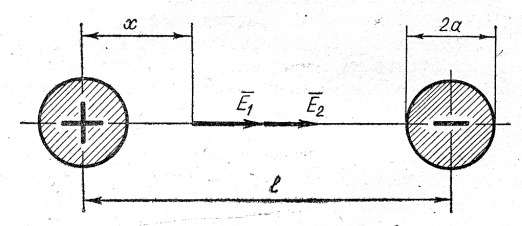
\includegraphics[height = 5cm]{example.png}
  \caption*{Вид рассматриваемой системы}
\end{figure}
Рассмотрим случай $l \gg a$. Напряженность поля в какой"=либо точке $x$ на выбранной линии сложится из напряженности 
$$
  E_1 = \frac{\lambda}{2\pi\epsilon_0} \cdot \frac{1},{x}
$$
создаваемой положительным проводом, и напряженности 
$$
  E_2 = \frac{\lambda}{2\pi\epsilon_0} \cdot \frac{1}{l - x}
$$
отрицательно заряженого провода; здесь $\lambda$ "--- заряд на единицу длины провода. Таким образом
$$
  E(x) = E_1 + E_2 = \frac{\lambda}{2\pi\epsilon_0}\Bigl(\frac{1}{x} + \frac{1}{l - x}\Bigr)
$$
Разность потенциалов между левым проводом и точкой $x$:
\begin{align*}
  \varphi = \int_{a}^{x} E(x)dx = \frac{\lambda}{2\pi\epsilon_0}\Bigl(\int_{a}^{x} \frac{dx}{x} + \int_{a}^{x}\frac{dx}{l - x}\Bigr) = \\
  = \frac{\lambda}{2\pi\epsilon_0}\Bigl(\ln{\frac{x}{a}} - \ln{\frac{l - x}{l - a}}\Bigr) = \frac{\lambda}{2\pi\epsilon_0}\Bigl(\ln{\frac{x}{l - x}} + \ln{\frac{l - a}{a}}\Bigr)
\end{align*}

Полная разность потенциалов между проводами
\begin{align*}
  \varphi = \int_{a}^{x} E(x)dx = \frac{\lambda}{\pi\epsilon_0}\, \ln{\frac{l - a}{a}}
\end{align*}

Относительный потенциал в точке
\begin{equation*}
  \frac{\varphi(x)}{\varphi_0} = \frac{\ln{\frac{x}{l - x}} + \ln{\frac{l - a}{a}}}{2\ln{\frac{l - a}{a}}}  
\end{equation*}


\section*{Эксперементальная часть}

В работе на электролитической ванне исследуются двумерные электростатические поля, создаваемые электродамаи различной конфигурации с заданными потенциалами. Эксперементально определяются эквипотенциальные линии, характеризующие исследуемое электрическое поле.

Ванна, на которой проводятся измерения, изготовлена из материала с хорошими изолирующими свойствами и содержит набор разнообразных электродов, укрепленныз на ее дне. Каждый из электродов имеет вывод на соответствующую клемму. 

При использовании жидкого электролита источником ошибок в экспериментах является система питания электродов напряжением постоянного тока вследствие возникновения электролиза, что приводит к нарушению однородности электролита и поляризации электродов. Во избежание этого электроды запитываются переменным напряжением от звукового генератора. При этом все предыдущие условия моделирования, которые были сформулированы для постоянно тока, остаются в силе и для переменного тока, если выполняются условия квазистационарности, которые означают, что размеры рассматриваемой системы электродов малы по сравнению с длиной электромагнитной волны, соответствующей рабочей частоте генератора. Чем меньше частота переменного напряжения (больше длина волны), тем точнее выполняются условия квазистационарности.

Напряжение, снимаемое с выхода звукового генератора, подается одновременно на электроды модели и делитель, состоящий из магазинов сопротивлений со ступенчатым переключением на 10 положений.

Напряжение, подаваемое на электроды, выбирается таким, чтобы при измерениях обеспечивалась достаточная чувствительность схемы. При снятии картины поля условно примем потенциал одного электрода за $0$, другого за $100\%$. Для однозначности результатов измерений следует устанавливать показания сопротивлений таким образом, чтобы всегда в процессе работы суммарное сопротивление левого и правого плечей оставалось постоянным. Варьируя величинами сопротивлений делителя, удается задать на зонд любой необходимый потенциал относительно электродов, расположенных в ванее, помня о том, что сумма показания делителей в сумме должны всегда составлять $100\%$.

Процесс изучения поля исследуемой модели сводится к следующему. Лист бумаги помещают на стеклянном столе ванны над той моделью, которая является объектом изучения. Место соприкосновения острия зонда с поверхностью воды проектируется на бумагу с помощью светового <<зайчика>> крестообразной формы. Центр креста соответствует острию зонда. Сначала наносят на бумагу форму электродов изучаемой модели. Затем с помощью делителя на зонд подается соответствующий потенциал равный, например, $10\%$ от общего напряжения на электродах модели. Устанавливают необходимую амплитуду выходного сигнала звукового генератора. В качестве индикатора в цепь зонда вклюачется электронный осциллограф. Величина сигнала на осциллографе зависит от того, в какой точке изучаемого поля находится зонд. Если зонд находтится в той точке поля, потенциал которого равен потенциалу, заданному делителем, то, очевидно, сигнал, подаваемый на вход осциллографа, будет равен нулю (или, по крайней мере, наименьшим). Любое перемещение зонда в другую точку поля приводит к увеличению сигнала на осциллографе. Итак, по наименьшому сигналу на осциллографе легко находятся точки поля с потенциалом, установленным на делителе. Геометрическое место точек с одинаковым потенциалом образует эквипотенциальную поверхность . Задавая на делителе различные значения потенциала, удается получить картину эквипотенциальных линий исследуемого макета. Около каждой эквипотенциальной линии записывают соответствующее ей значение потенциала в процентах.

Уровень воды в ванне должен быть таким, чтобы измерительный зонд погружался в воду на $2$--$3$ мм.

При выполнении работы запрещается касаться руками электродов и зонда, расположенных в ванне. Перемещение зонда осуществлять только с помощью специального устройства, изолированного от электролита прозрачным диэлектриком.

В ходе работы мы исследовали три электростатических поля, создаваемые электродами различной конфигурации. Исследования отражены на листах №1, №2 и №3. Вдоль каждой эквипотенциальной линии записано отношение сопротивлений.

В листе №3 вычислим относительный потенциал в точке.

Радиус цилиндра $a = 0,75$ см. Для выбранной точки расстояние между электродами $l = 5,8$ см, расстояние от плоского электрода до точки $x = 1,9$ см.

Воспользуемся формулой 
\begin{align*}
  \frac{\varphi(x)}{\varphi_0} = \frac{\ln{\frac{x}{l - x}} + \ln{\frac{l - a}{a}}}{2\ln{\frac{l - a}{a}}}
\end{align*}
где $\varphi_0$ "--- полная разность потенциалов между проводами.
Подставим:
\begin{align*}
  \frac{\varphi(x)}{\varphi_0} = \frac{\ln{\frac{1,9}{5,8 - 1,9}} + \ln{\frac{5,8 - 0,75}{0,75}}}{2\ln{\frac{5,8 - 0,75}{0,75}}}
\end{align*}
$$
\frac{\varphi(x)}{\varphi_0} \thickapprox 0,31
$$

Возьмём потенциал верхнего электрода за $0\%$, а другой за $100\%$, тогда $\varphi_0 = 100\%$. Для данной точки отношение сопротивлений равно $7/3$, то есть
$$
  \frac{\varphi(x)}{\varphi_0} = \frac{3}{10} = 0,30
$$

Оценим погрешность:
$$
  \frac{0,31 - 0,3}{0,31} \cdot 100\% \thickapprox 3,2\%
$$

\section*{Вывод}
Ознакомившись с методом моделирования электростатического поля на электролитической ванне, получили для различных пар электродов электростатические поля. Вычислили относительный потенциал в точке и сравнили его с эксперементальными данными. Погрешность может появляться из"=за человеческого фактора и погрешностей аппаратуры.



% При исследовании поля плоского конденсатора снять эквипотенциальные линии через каждые $10\%$ изменения потенциала. Построить теоретическую зависимость распределения потенциала (в относительных единицах) между пластинами. На этот же график нанести эксперементальные точки, полученные из анализа снятой картины поля.